\chapter{Réalisation du système (Secure Requirements Studio)}
\markboth{CHAPITRE 4. RÉALISATION DU SYSTÈME~--~SRS}{CHAPITRE 4. RÉALISATION DU SYSTÈME~--~SRS}

\section{Introduction}

Ce quatrième chapitre concrétise les phases précédentes d'analyse et de conception en présentant la réalisation effective de notre application logicielle \textbf{Secure Requirements Studio (SRS)}, dédiée à l'ingénierie des exigences et à la formalisation du Cahier des Charges. Nous y décrivons l'environnement matériel et logiciel ayant servi au développement, détaillons les choix technologiques retenus, et présentons une revue complète des véritables interfaces graphiques de l'application. Enfin, nous analysons le livrable de référence généré par le système, le document officiel \texttt{Cahier\_des\_Charges\_FOCP\_V3.pdf}, qui sert de socle à la réalisation du prototype fonctionnel présenté au chapitre suivant.

\section{Environnement de développement}

\subsection{Environnement matériel}

Le développement, les tests et l'intégration continue de l'application SRS ont été réalisés sur une station de travail standard d'ingénierie logicielle dotée d'une architecture multi-coeurs x86-64, d'une mémoire vive suffisante pour l'exécution simultanée des conteneurs Docker (PostgreSQL, serveurs applicatifs) et d'un stockage SSD garantissant des temps d'exécution et de compilation optimaux.

\subsection{Environnement logiciel}

L'écosystème technologique retenu regroupe des outils et frameworks modernes et performants :

\begin{itemize}
    \item \textbf{Système d'exploitation et contrôle de version} : Environnement Windows avec terminal PowerShell, gestionnaire de versions Git et hébergement du code sur GitHub.
    \item \textbf{Framework Backend (FastAPI / Python 3.12)} : Framework web asynchrone à haute performance, sélectionné pour sa rapidité d'exécution, sa documentation OpenAPI interactive et son intégration native de Pydantic v2 pour la validation stricte des schémas de données.
    \item \textbf{Couche de persistance et ORM (SQLAlchemy 2.0 \& Alembic)} : Mapping objet-relationnel asynchrone (\texttt{asyncpg} pour PostgreSQL et \texttt{aiosqlite} pour l'environnement local), complété par Alembic pour les migrations de schéma.
    \item \textbf{Framework Frontend (Next.js 15 \& React 19)} : Framework JavaScript/TypeScript exploitant l'architecture \textit{App Router}, le rendu côté serveur optimisé et un typage statique de bout en bout.
    \item \textbf{Design System et Styling (Tailwind CSS v4 \& Framer Motion)} : Conception d'une interface responsive et soignée avec gestion dynamique des thèmes sombre et clair.
    \item \textbf{Moteur d'IA et SDK Cloud (Google GenAI SDK)} : Intégration du SDK officiel pour l'assistance contextuelle lors de l'entretien d'élicitation adaptatif via les modèles Google Gemini.
    \item \textbf{Moteurs de rendu documentaire} : Bibliothèque ReportLab pour la génération du format PDF, \texttt{python-docx} pour le format Word, et parseur Markdown2 pour les formats balisés.
    \item \textbf{Conteneurisation (Docker \& Docker Compose)} : Orchestration multi-services isolant le frontend, le backend et la base de données relationnelle.
\end{itemize}

\section{Principales interfaces graphiques de l'application SRS}

Nous présentons ci-après les véritables captures d'écran illustrant le parcours utilisateur au sein de notre application logicielle de formalisation des exigences.

\subsection{Accueil et sélection du mode de création}

L'interface d'accueil (figure \ref{fig:srs_01_accueil}) accueille l'analyste et lui propose d'orienter le projet dès son initialisation entre deux démarches d'élicitation distinctes : le \textbf{Mode 1 (Questionnaire guidé classique)}, structuré en étapes thématiques déterministes, et le \textbf{Mode 2 (AI Interview)}, interactif et adaptatif, exploitant la puissance d'analyse du grand modèle de langage Google Gemini.

\begin{figure}[H]
\centering
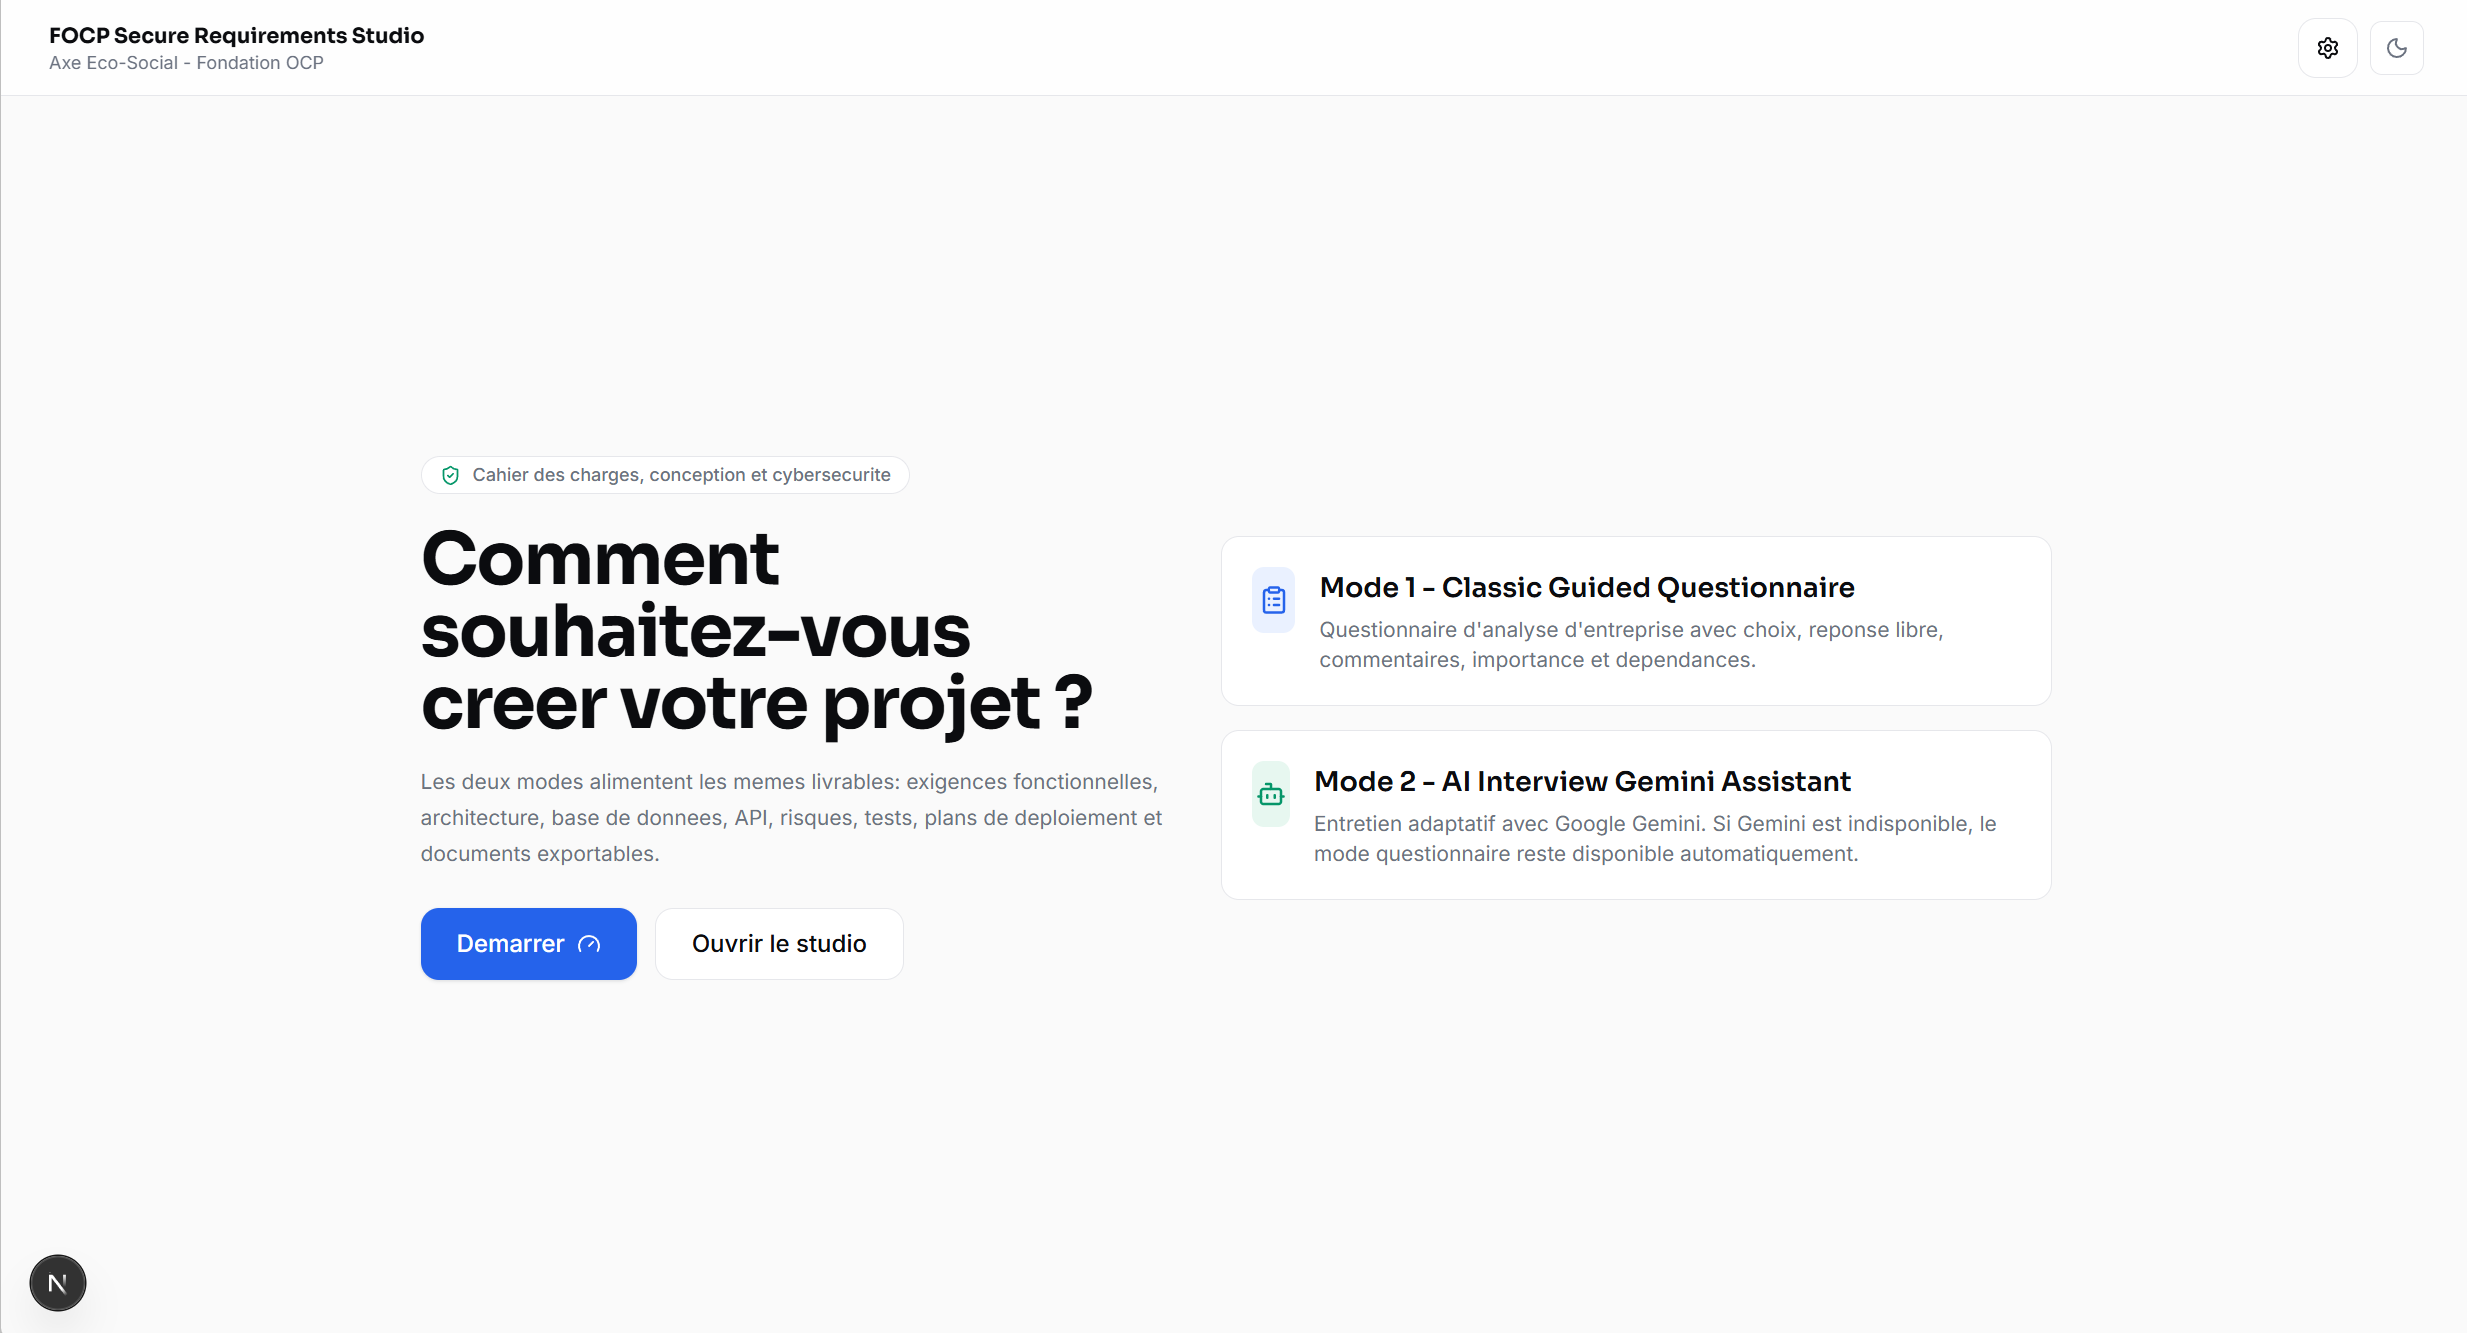
\includegraphics[width=0.92\textwidth]{figures/screenshots/srs/01_srs_accueil_mode.png}
\caption{Interface d'accueil et sélection du mode d'élicitation de projet}
\label{fig:srs_01_accueil}
\end{figure}

Cette vue permet de lancer un nouveau projet ou de charger un projet existant tout en rappelant le contexte institutionnel de la Fondation OCP.

\subsection{Formulaire d'initialisation d'un nouveau projet}

L'interface de création (figure \ref{fig:srs_02_projet}) permet de renseigner les métadonnées administratives essentielles : nom complet du projet, sigle court, direction commanditaire (Axe Social et Solidaire / DTD) et description générale du périmètre.

\begin{figure}[H]
\centering
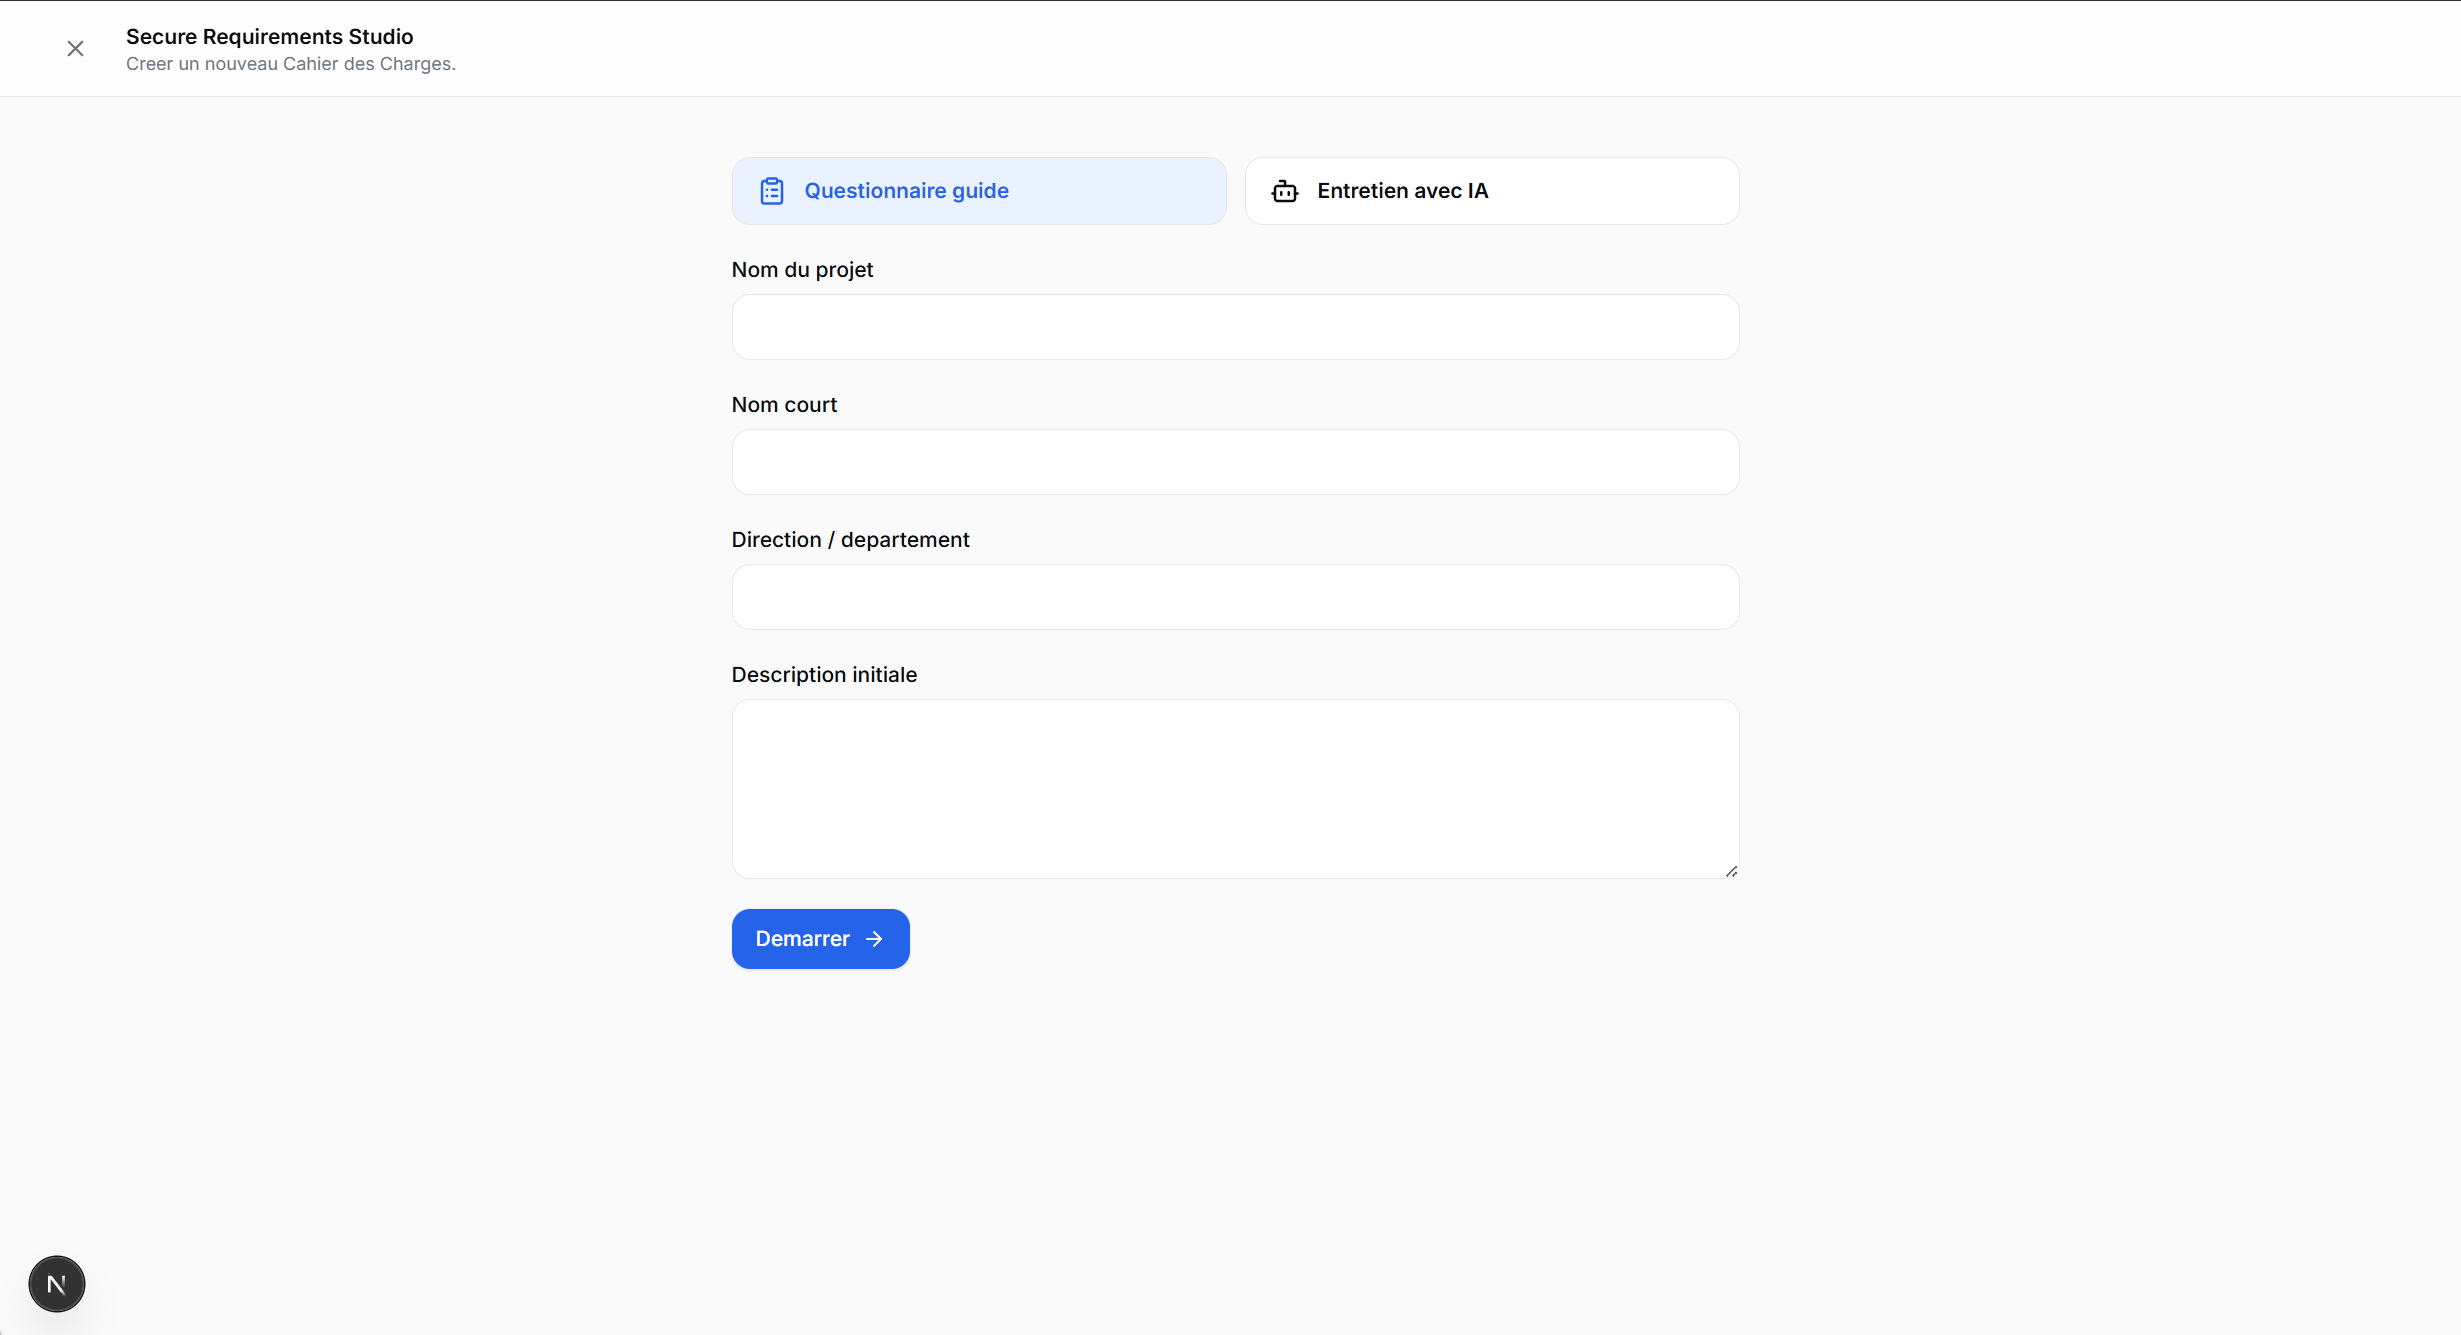
\includegraphics[width=0.92\textwidth]{figures/screenshots/srs/02_srs_nouveau_projet.png}
\caption{Formulaire d'initialisation et de paramétrage d'un nouveau projet}
\label{fig:srs_02_projet}
\end{figure}

La validation de ce formulaire instancie automatiquement en base de données le graphe de connaissances ontologique initialisé avec ses 39 concepts clés.

\subsection{Tableau de bord principal de pilotage des projets}

Le tableau de bord central (figure \ref{fig:srs_03_dashboard}) offre une vue panoramique de l'ensemble des projets de spécification initiés. Il met en avant les indicateurs de synthèse (nombre de projets, taux de complétude, score de sécurité moyen, total des exigences dérivées) ainsi que la liste détaillée des projets avec leur statut de cadrage.

\begin{figure}[H]
\centering
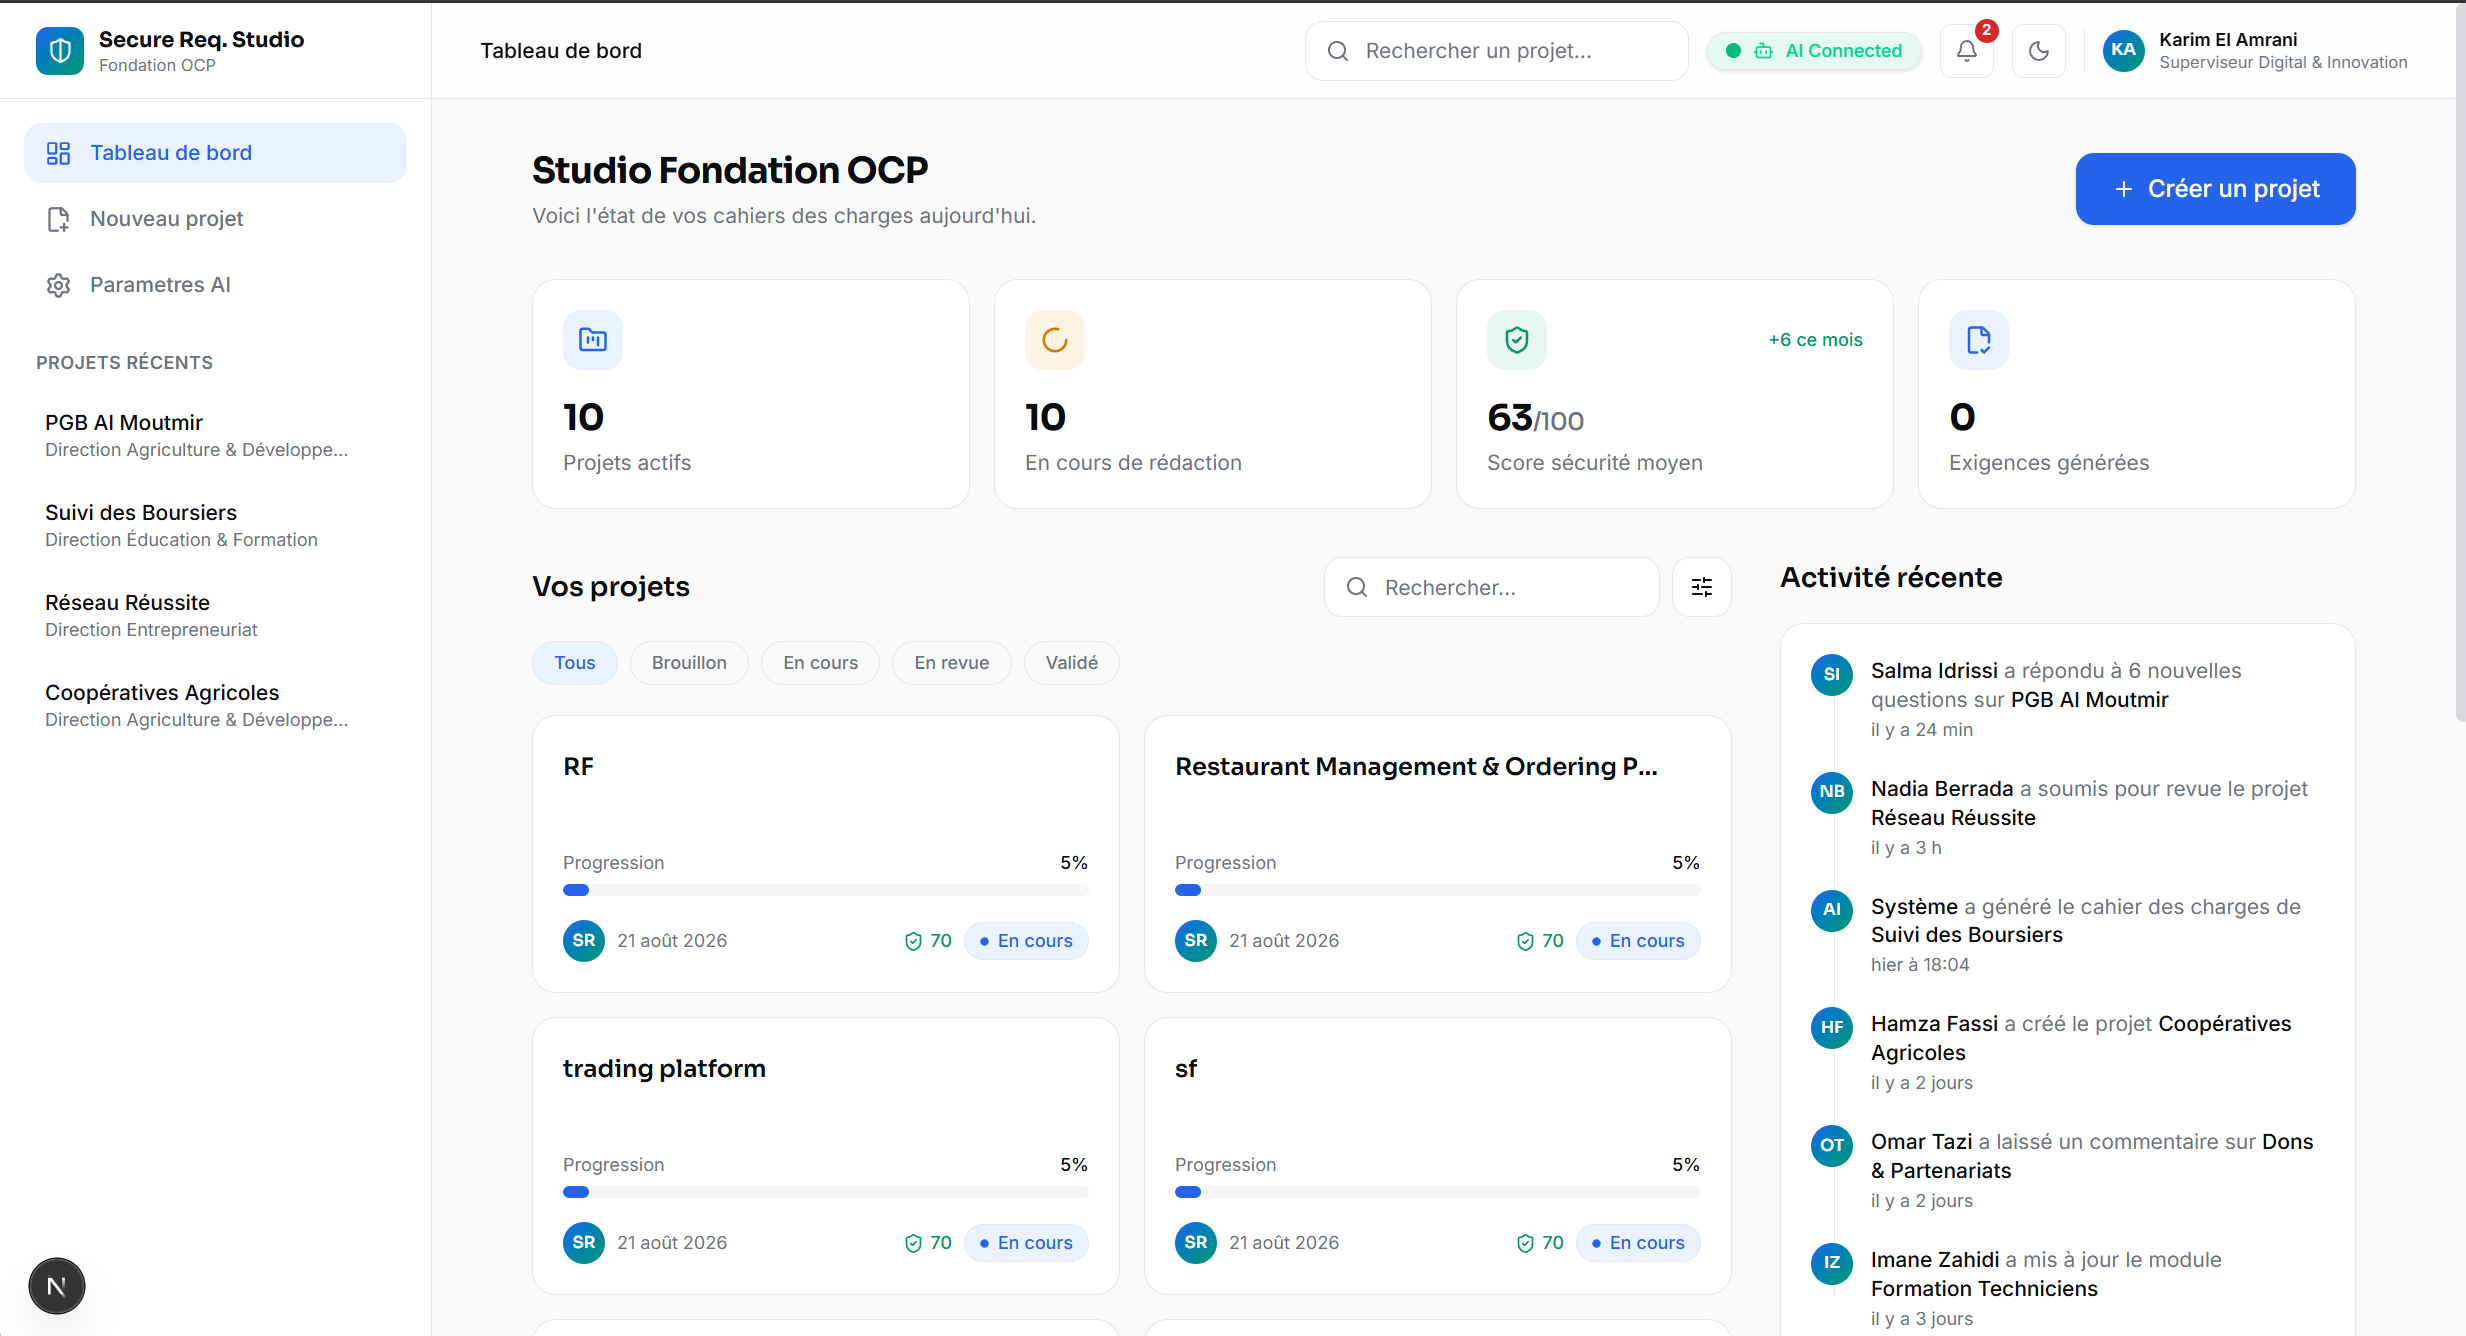
\includegraphics[width=0.92\textwidth]{figures/screenshots/srs/03_srs_dashboard.png}
\caption{Tableau de bord de supervision et de pilotage des projets de spécification}
\label{fig:srs_03_dashboard}
\end{figure}

L'analyste dispose ici d'une visibilité directe sur la maturité de chaque dossier et peut accéder aux actions de reprise d'interview, d'audit ou d'exportation.

\subsection{Paramètres et configuration des fournisseurs d'intelligence artificielle}

L'interface des paramètres (figure \ref{fig:srs_04_params}) permet de configurer les clés d'authentification API et de sélectionner le modèle de langage actif (Google Gemini 1.5 Pro ou Gemini 1.5 Flash).

\begin{figure}[H]
\centering
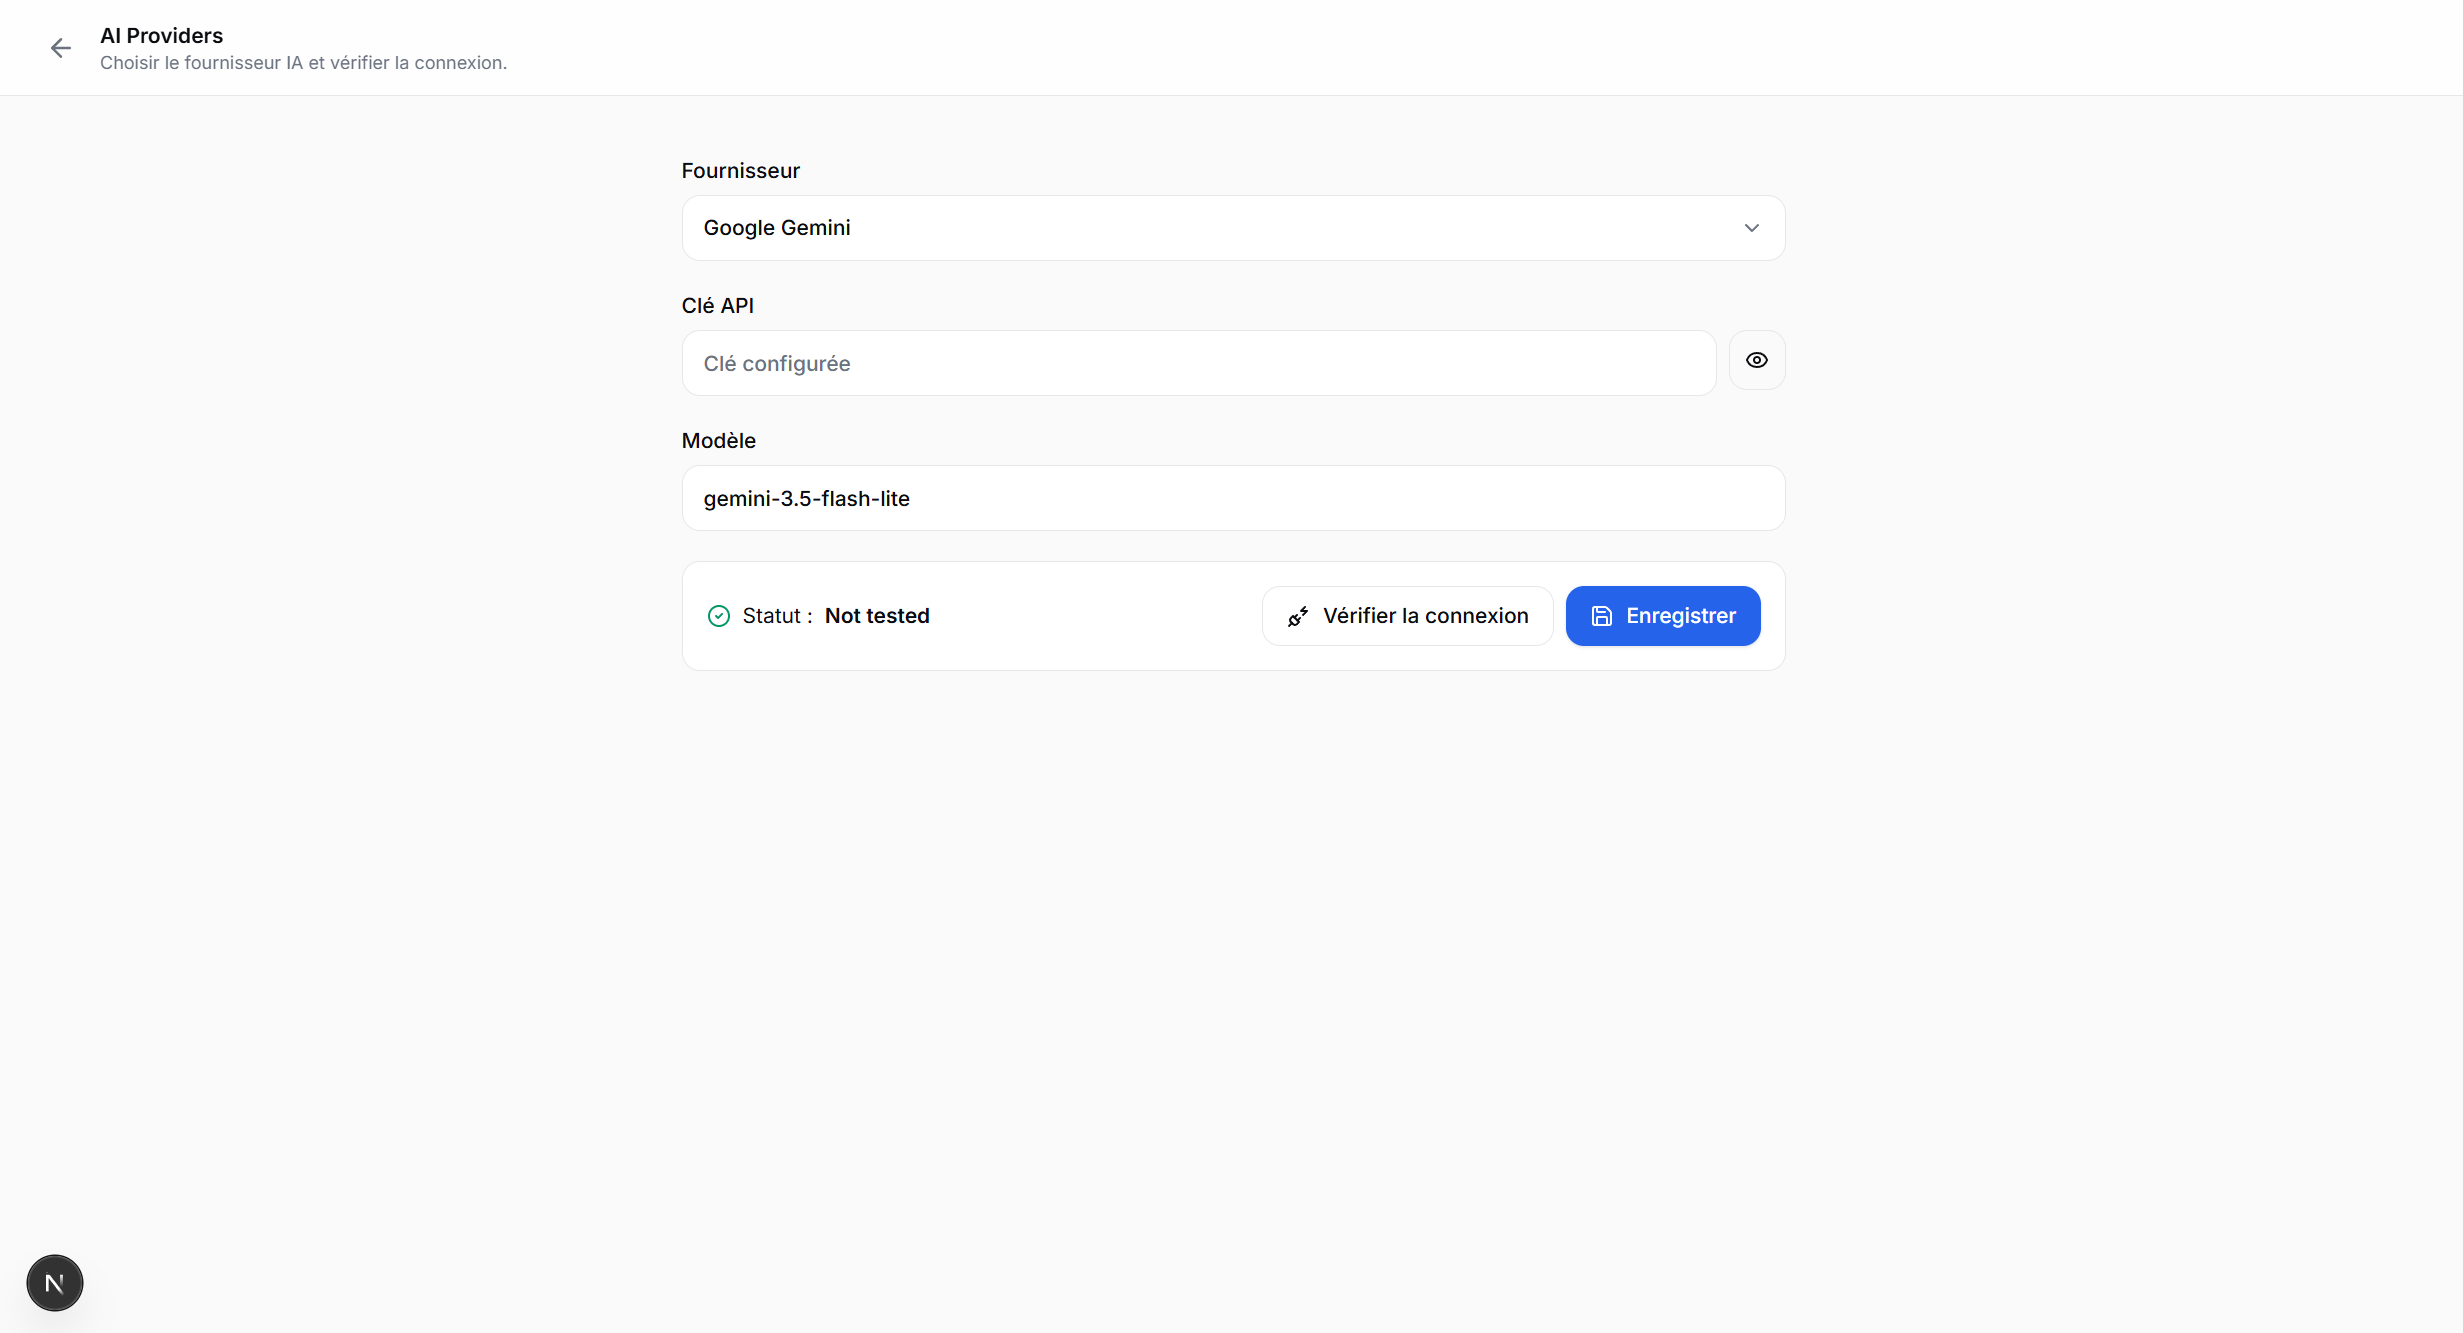
\includegraphics[width=0.92\textwidth]{figures/screenshots/srs/04_srs_parametres_ia.png}
\caption{Interface de configuration des fournisseurs d'IA et clés d'API (Google Gemini)}
\label{fig:srs_04_params}
\end{figure}

Ce paramétrage assure la flexibilité du système et garantit le basculement transparent vers le moteur déterministe local en cas de non-renseignement de clé d'API.

\subsection{Questionnaire guidé par étapes d'élicitation}

Le module d'interview guidée (figure \ref{fig:srs_05_questionnaire}) structure la capture des besoins selon une progression séquentielle par domaines : Contexte global, Utilisateurs \& Rôles, Fonctions métier, Processus \& Workflows, Contraintes techniques, Sécurité \& Priorités.

\begin{figure}[H]
\centering
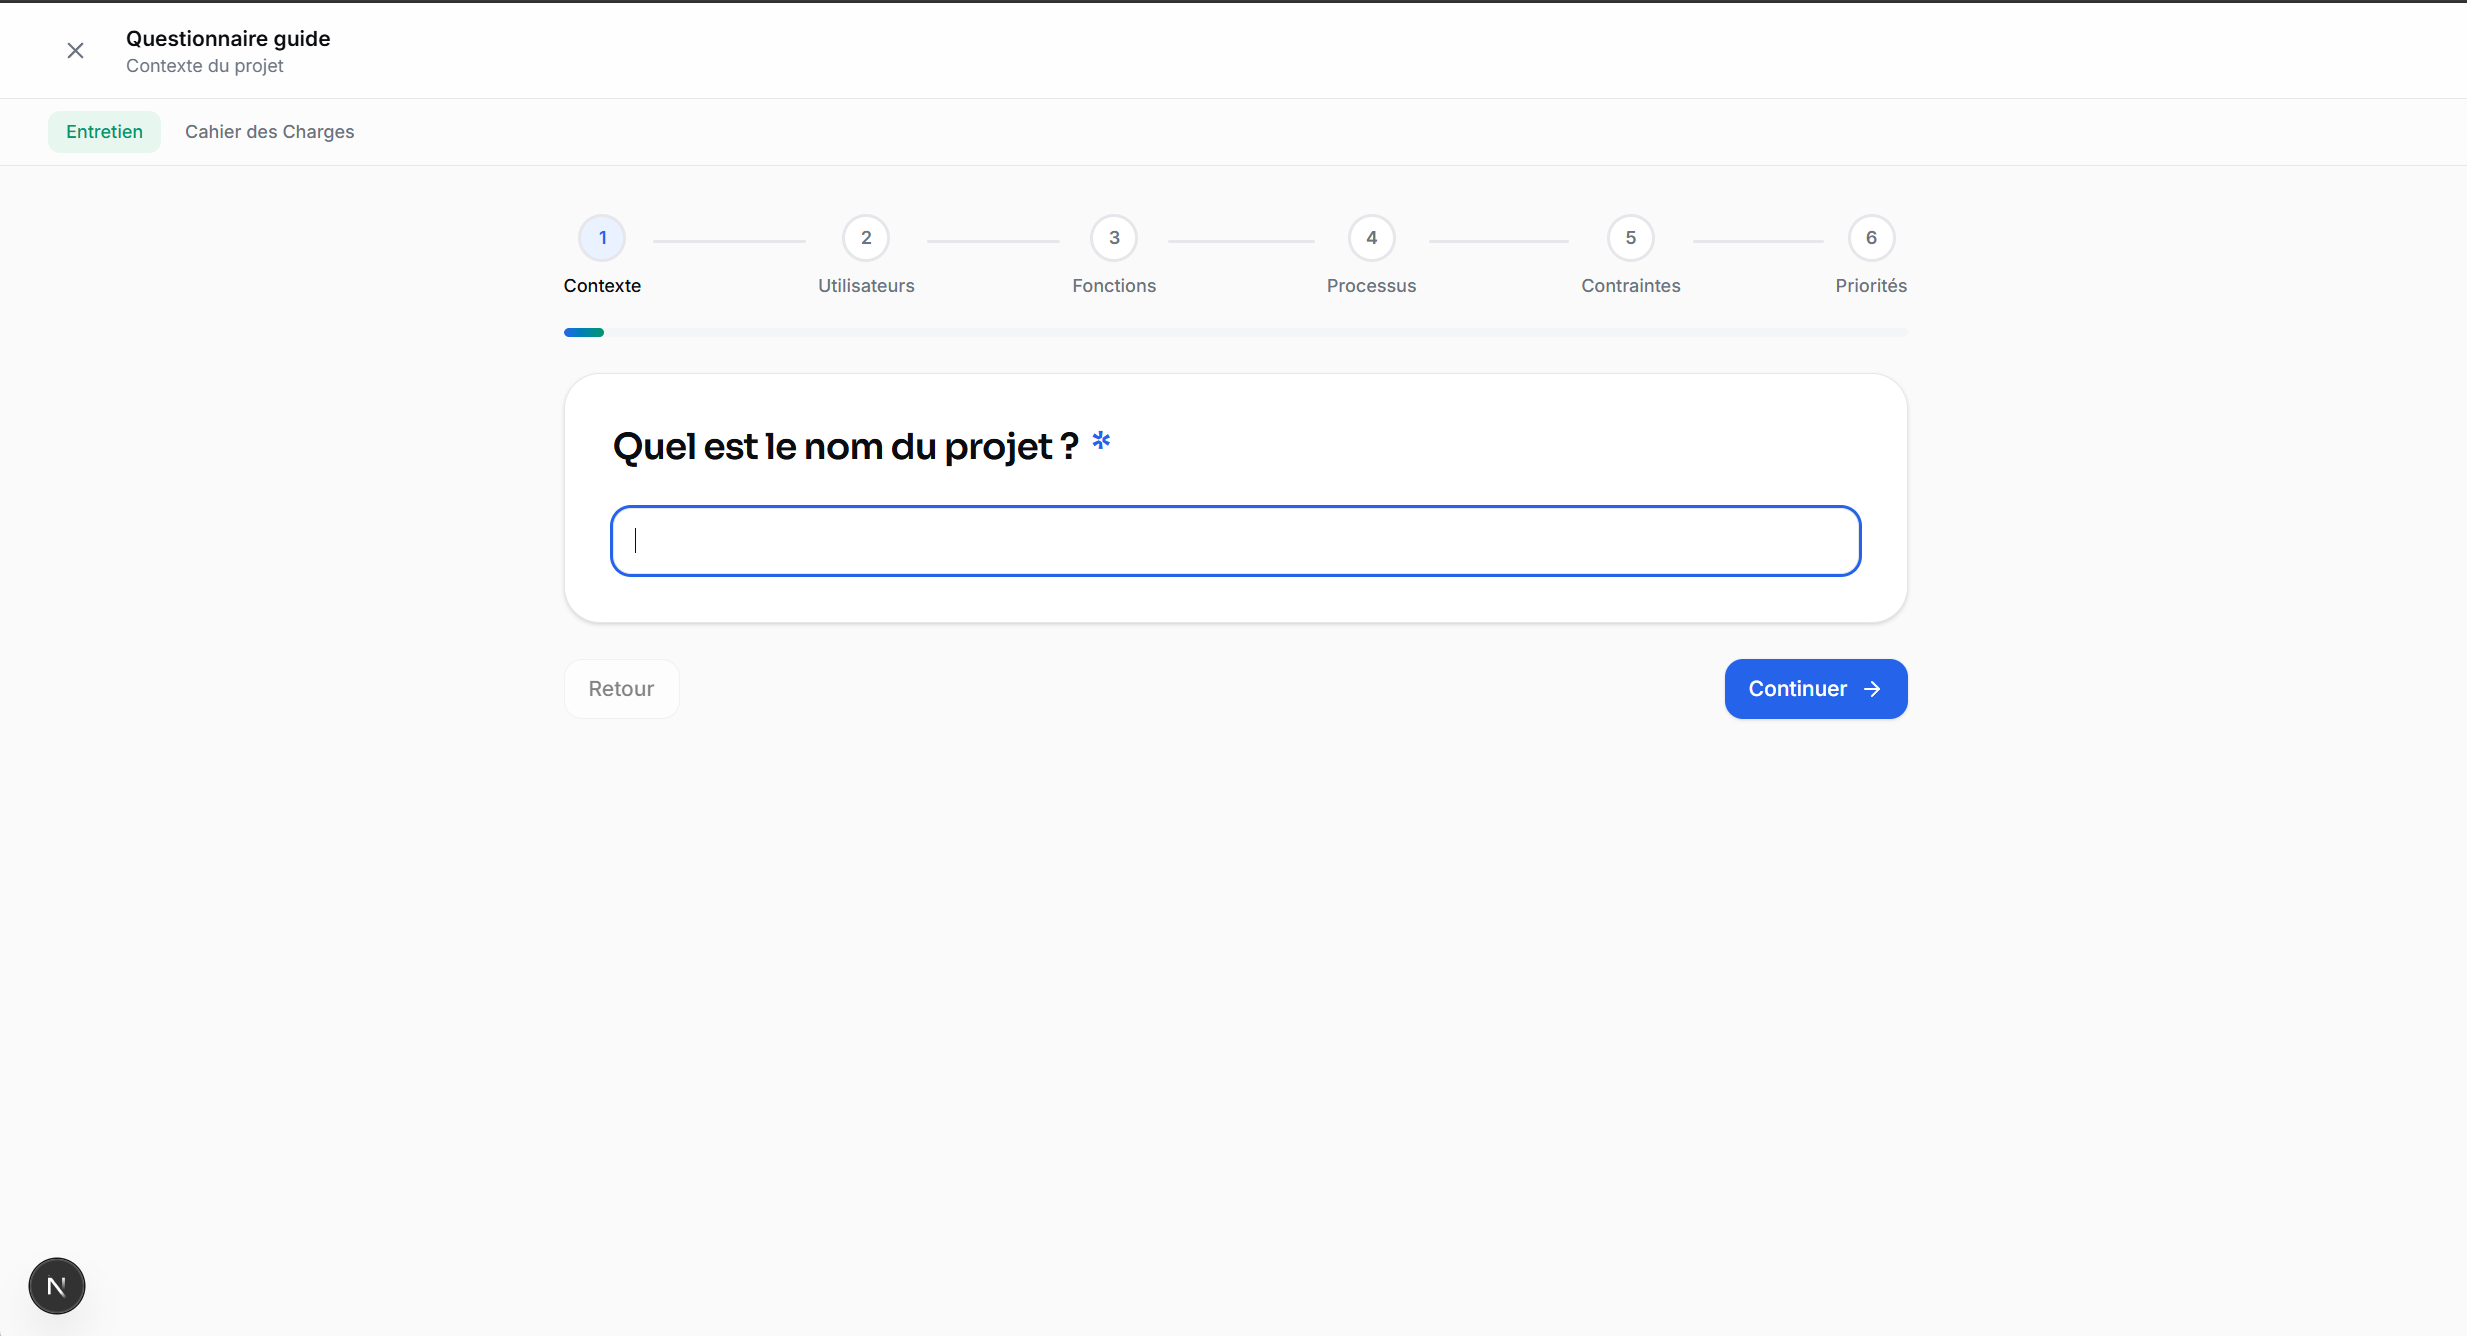
\includegraphics[width=0.92\textwidth]{figures/screenshots/srs/05_srs_questionnaire_guide.png}
\caption{Interface du questionnaire d'élicitation structuré par étapes thématiques}
\label{fig:srs_05_questionnaire}
\end{figure}

Chaque réponse validée par l'analyste déclenche une mise à jour instantanée du graphe conceptuel et la dérivation dynamique des exigences fonctionnelles et de sécurité associées.

\subsection{Prévisualisation du Cahier des Charges généré}

L'interface de prévisualisation (figure \ref{fig:srs_06_preview}) permet de visualiser en direct la structure complète du document de spécification assemblé par le moteur documentaire.

\begin{figure}[H]
\centering
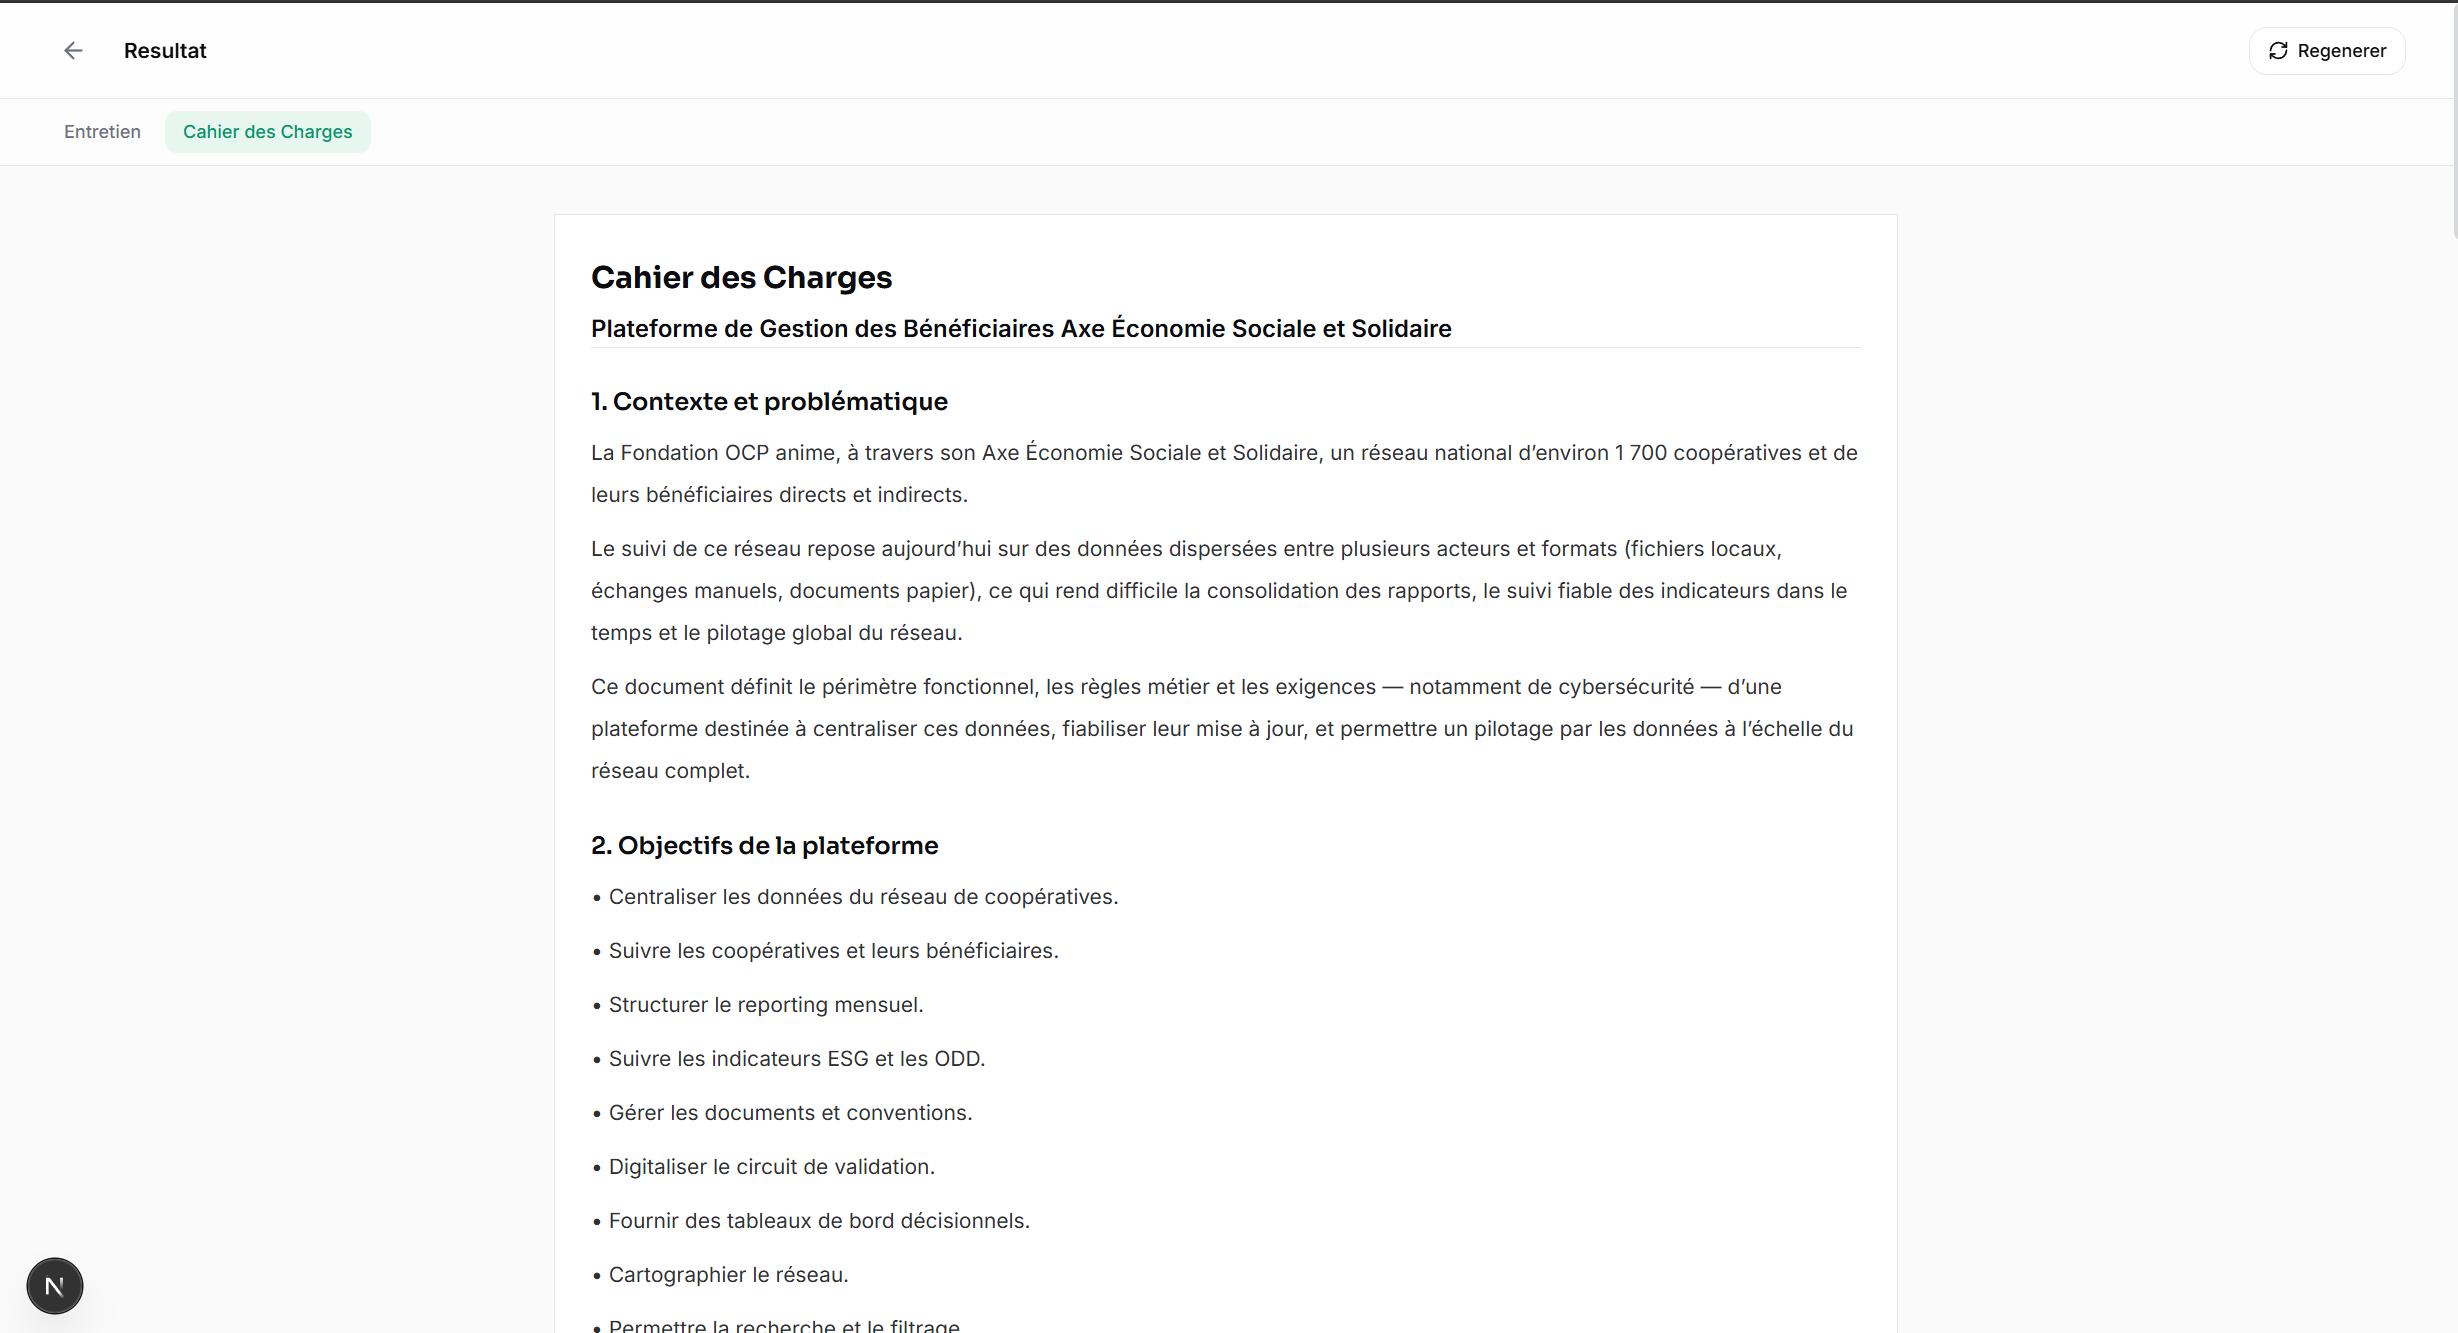
\includegraphics[width=0.92\textwidth]{figures/screenshots/srs/06_srs_cahier_charges_preview.png}
\caption{Interface de prévisualisation interactive du Cahier des Charges assemblé}
\label{fig:srs_06_preview}
\end{figure}

L'utilisateur y vérifie l'articulation entre les objectifs stratégiques, les profils d'utilisateurs RBAC, les entités manipulées et les critères d'acceptation avant d'engager le téléchargement dans le format de son choix (PDF, DOCX, Markdown, LaTeX).

\subsection{Résumé et analyse de maturité du projet}

L'interface de synthèse (figure \ref{fig:srs_07_resume}) dresse le bilan d'évaluation du projet : état d'homologation, score de cybersécurité calculé, modules fonctionnels détectés et rôles identifiés.

\begin{figure}[H]
\centering
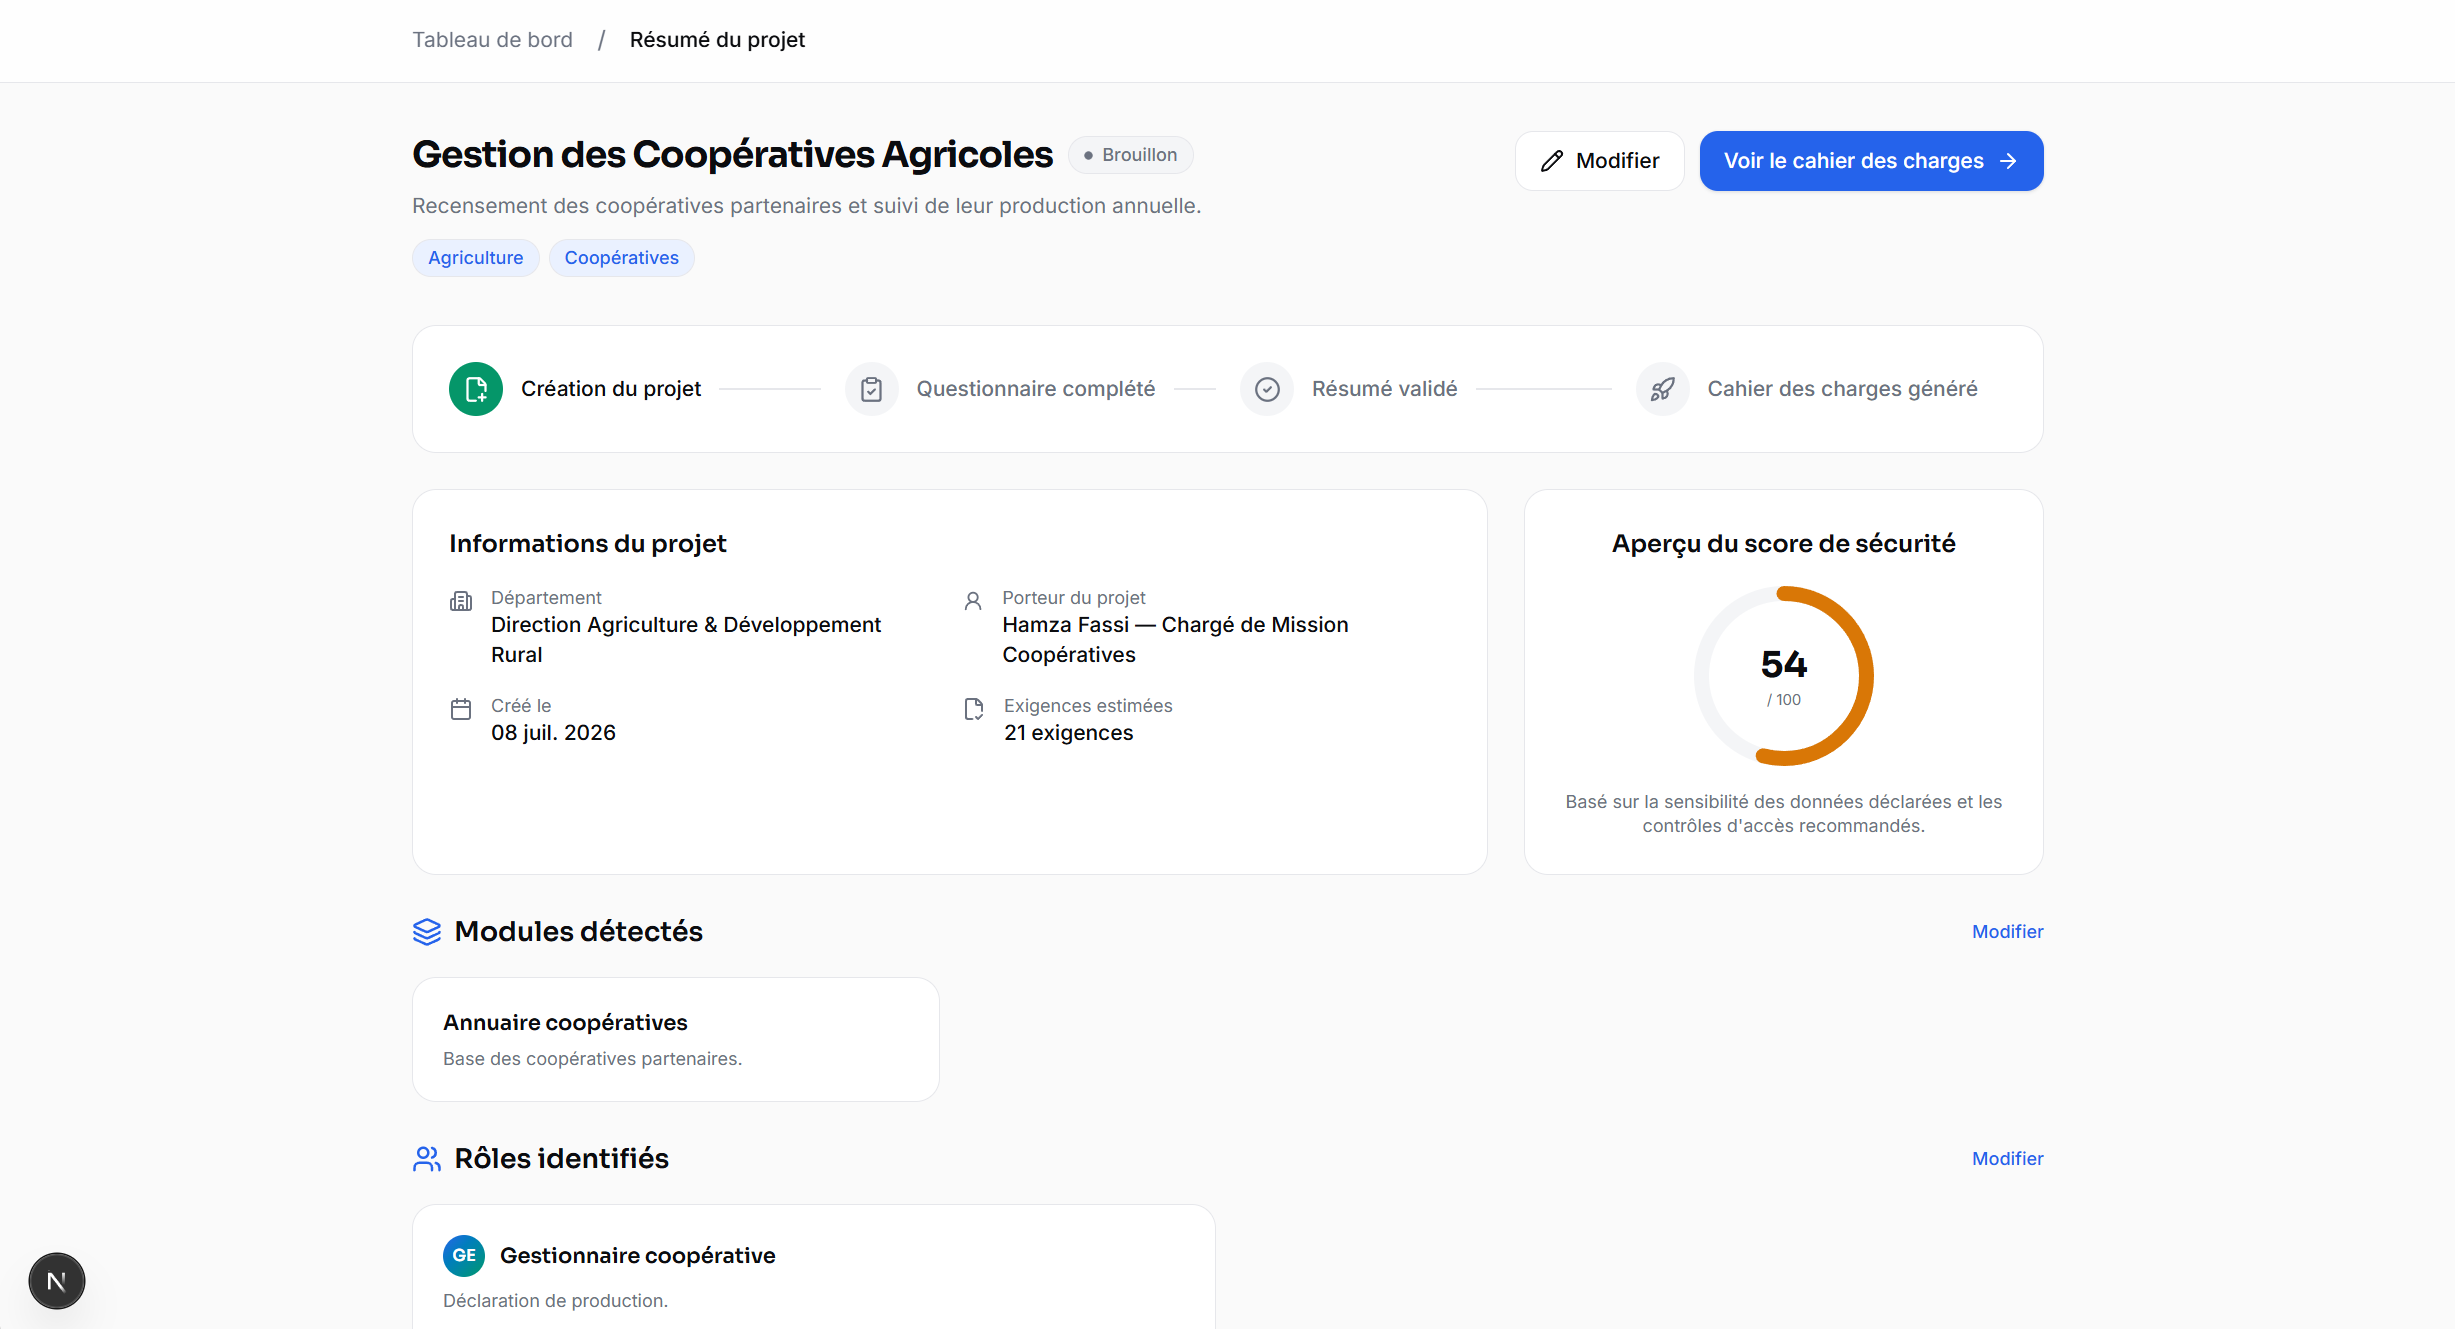
\includegraphics[width=0.92\textwidth]{figures/screenshots/srs/07_srs_resume_projet.png}
\caption{Interface de synthèse du projet : statut, score de sécurité et modules détectés}
\label{fig:srs_07_resume}
\end{figure}

Cette vue fournit une traçabilité complète permettant d'attester que le dossier de spécification a atteint le niveau de qualité requis pour engager la phase de réalisation.

\section[Analyse du livrable final : Cahier des Charges FOCP V3]{Analyse du livrable final~: {\ttfamily Cahier\allowbreak\_\allowbreak des\allowbreak\_\allowbreak Charges\allowbreak\_\allowbreak FOCP\allowbreak\_\allowbreak V3.pdf}}

L'aboutissement opérationnel direct de notre application logicielle SRS est la production du document officiel de référence : {\ttfamily Cahier\allowbreak\_\allowbreak des\allowbreak\_\allowbreak Charges\allowbreak\_\allowbreak FOCP\allowbreak\_\allowbreak V3.pdf}.

Ce livrable formalise l'intégralité des spécifications de la future \textbf{plateforme de gestion des bénéficiaires de l'Axe Social et Solidaire au sein de la Fondation OCP en intégrant des exigences de cybersécurité}. L'analyse de sa structure révèle les sections majeures générées automatiquement par notre système :
\begin{enumerate}
    \item \textbf{Contexte et problématique} : Définition du réseau de 1\,700 coopératives et justification du besoin de centralisation et de sécurisation des données.
    \item \textbf{Objectifs de la plateforme} : 12 objectifs stratégiques (centralisation, reporting mensuel, indicateurs ESG/ODD, gestion documentaire, cartographie, traçabilité, cybersécurité).
    \item \textbf{Utilisateurs et permissions (RBAC)} : Définition stricte des rôles \textit{Administrateur Fondation OCP} (accès global, analyse, validation, correction exceptionnelle tracée) et \textit{Représentant de coopérative} (accès limité à son profil, déclaration des bénéficiaires et activités).
    \item \textbf{Données gérées} : Structuration des données des coopératives, bénéficiaires directs et indirects (femmes, jeunes, handicap, agriculteurs), activités, documents et conventions.
    \item \textbf{Workflow mensuel de soumission et validation} : Circuit digitalisé de saisie, soumission, validation ou rejet motivé avec notification et correction traçable.
    \item \textbf{Tableaux de bord et cartographie} : Spécification des KPI décisionnels et de la carte interactive géolocalisant les coopératives par région et province.
    \item \textbf{Exigences de cybersécurité transversales} : Contrôle d'accès RBAC, principe du moindre privilège, politique de mot de passe, chiffrement des données sensibles, validation des fichiers et journalisation systématique de toutes les opérations.
    \item \textbf{Critères d'acceptation et de validation} : Liste des critères d'homologation et points de décision soumis à arbitrage avec la Fondation.
\end{enumerate}

Ce livrable démontre la capacité de notre application logicielle SRS à transformer un processus d'élicitation complexe en un document de spécification hautement qualifié, rigoureux et prêt à l'emploi.

\section{Conclusion}

Ce chapitre a illustré la réalisation logicielle effective de l'application \textbf{Secure Requirements Studio (SRS)}. L'écosystème technologique moderne (FastAPI, Next.js 15, SQLAlchemy, Docker, Google Gemini) a permis d'implémenter avec succès les modules de capture ontologique, d'analyse de cybersécurité, d'audit qualité et d'assemblage documentaire. Cette chaîne a permis de produire le document officiel {\ttfamily Cahier\allowbreak\_\allowbreak des\allowbreak\_\allowbreak Charges\allowbreak\_\allowbreak FOCP\allowbreak\_\allowbreak V3.pdf}.

Afin de concrétiser ces spécifications et d'en valider l'opérabilité par une preuve de concept concrète, nous avons développé le prototype fonctionnel (MVP) de la plateforme de gestion des bénéficiaires, dont la réalisation et les interfaces détaillées font l'objet du chapitre 5 suivant.

\newpage
